\section{Concepts}


\subsection{Glossary}

\textbf{Symbiosis: }

Circular Economy

Sharing Economy

Industrial Synergy

Agent-Based Model

Complex System

Internet of Things


Industrial Ecology
Material Flow Analysis


Sustainable Development Goals


United Nations


Industrial Symbiosis Dynamics

Cleaner production


Product-service systems (PSS) are

Bounded rationality

Embeddedness

Eco-Industrial Parks

Life cycle assestment

Material flow analysis
circular business models (CBMs) 

Resilience

Sustainability

by-product synergy (BPS)

Local Authorities

Public Private Partnership PPP

Place promotion or ‘boosterism’ (Short, 1999; Prytherch, 2002)


Closed loop 

Sustainable development

Local Agenda 21

Zero Waste Manufacturing 

Emergy is a measure of real wealth, defined as “the sum of available energy of one kind previously required directly and indirectly through input pathways to make a product or service”

3Rs (recycle, reduce and reuse)
Resource recovery (RR)
In-house reuse

Cost-Benefit analysis

Institutional capacity

Industrial poles

Industrial Symbiosis Network
Resilence

sustainable production and consumption (SPC)
triple-bottom-line (TBL) decision-making
institutional capacity building.

By-product synergy (BPS) : It consists in the maximization of resources utilization with the replacement of raw materials by by-products as inputs for industrial processes. In

Sustainability-Oriented Cooperation

\subsection{Methods}
MIND Method -> Method for analysis of INDus-
trial energy systems [18,19]. It is based on mixed integer linear programming (MILP) and has mainly been used for modelling industrial plants and to some extent for modelling the interac- tion between an industry and a district heating system [20,21].
(Karlsson2008)

\subsection{Case studies}
\textbf{Tampico, Mexico}
Midong Chemical Industrial Park (MCIP), China
Kalundborg, Denmark
Viotia region, Greece
Kawasaki’s experience JPN IRON/STEEL

Jinan and Liuzhou of China
Liuzhou city
Liuzhou and Jinan Liang, China - IRON/STEEL
Handelo bioenergy complex, Norrkoping, Sweden
Barceloneta, Puerto Rico. 
recycling network Styria in Austria, 
recycling network Oldenburger Munsterland in Germany
manufacturing sector in Austria

Port of Cape Charles Sustainable Technology Park, USA
Devens Planned Community, USA
Londonderry Ecological Industrial Park, USA
Avtex Redevelopment Site, USA

Santa Croce sull’Arno

Tianjin Binhai New Area, China -> TEDA


Shandong Lubei eco-industrial park, china


\subsection{programmes}
\textbf{The Business Council for Sustainable Development, United Kingdom
national IS programme (NISP)}

Korean eco-industrial park scheme

Landskrona industrial symbiosis programme

Jiayuguan city is located in the western of China, which is a modern city that developed on the basis of Jiuquan Iron \& Steel Co., Ltd. (JISCO)

e-Symbiosis, Greece






\section{Research Aim and Objectives}































\subsection{General}
\textbf{\citetitle{Chertow2012}}\par
\textcite{Chertow2012} presents a discontinuous three-stage model used to describe the genesis of the process. While there is much variation, with no single path to this outcome, the recognition of benefits is seen as an emergent property characteristic of these self-organized systems that move beyond the initial stage. \par
-> Examples of 10 well-documented case studies \par
-> We do not yet have enough knowledge about industrial ecosystems to understand fully their life cycles and the categories into which they fall. Yet, what we are proposing moves beyond the biological notion of mutually beneficial exchange by two organisms toward network configurations involving many more. Specifically, the model they present applies to these 10 well-studied examples.


\begin{figure}[h!]
    \centering
    \includegraphics[width=0.85\textwidth]{Assets/Kalundborg.PNG}
    \caption{Evolution of industrial symbiosis of the Kalunborg region}
    \label{fig:Kalundborg}
\end{figure}


\textbf{\citetitle{Chertow2012}}\par
\textcite{Keckler1998} Linear and other mathematical programming approaches were used to evaluate water reuse opportunities. It is claimed that the methods used in this paper can be used to evaluate the potential reuse of other materials. \par
-> Case study of Bayport Facility:

\begin{figure}[h!]
    \centering
    \includegraphics[width=0.4\textwidth]{Assets/Bayport.PNG}
    \caption{Interaction of 3 manufacturers (M,O \& P) and 3 treatment steps (A, B \& C)}
    \label{fig:Bayport}
\end{figure}


\subsection{Industry 4.0}
\textbf{\citetitle{Kerdlap2019}}\par
\textcite{Kerdlap2019}, Zero Waste Manufacturing (ZWM) as a concept to help countries to support transition towards Circular Economy (CE). \par
The main focus is to eliminate waste across the entire supply chains.\par


\textbf{CASE STUDY:} Singapore\par
\textbf{CONTEXT:} Singapore lacks of land area to develop specific equipment which produces high prices. There is also a challenge of productivity and labor shortage.\par
\textbf{METHOD:} To identify the technologies that stakeholders can implement to achieve ZWM, this study proposes a holistic framework comprising six technology themes that aim to mitigate waste generation across the life cycle stages of production and consumption systems. These six themes include:\par

\begin{enumerate}
    \item design for zero waste
    \item smart waste audit and reduction planning
    \item smart waste collection
    \item high-value mixed waste processing
    \item collaborative platform for industrial symbiosis
    \item waste to resource conversion and recycling
\end{enumerate}\par

The authors identified the following benefits for each of the themes.
\begin{figure}[h!]
    \centering
    \includegraphics[width=0.8\textwidth]{Assets/s3.PNG}
    \caption{Stakeholders benefits under each theme of ZWM}
    \label{fig:ZWM}
\end{figure}

\textbf{RESULTS:} Main challenge for I.S. is to get a critical mass and be known\par

\textit{"Collaborative platforms for industrial symbiosis face few technical
barriers for implementation in Singapore. This technology relies primarily on digital systems and would require minimal to nearly no changes in physical infrastructure to implement (Yeo et al., 2019). Many sharing economy-based services are already actively used in Singapore and so a similar digital platform focused on waste to resource matching and exchanges between individuals and companies is technically feasible. One of the challenges that may arise during the initial stages of implementation would be achieving a critical mass of users for the collaborative platform to successfully facilitate industrial symbiosis exchanges. The impact on Singapore’s waste management system through implementing collaborative platforms for industrial symbiosis would be a reduction in the amount of waste materials that get mixed in with waste sent to incinerators. Instead, users would be directly matched to a market where their waste could be recycled to gain value and not need to rely on the existing waste collection and recycling system."} \par

Future research areas  6 identified:
\begin{enumerate}
    \item Smart bins that measure waste material composition:  
    \item Small and medium sized waste sorting technologies: 
    \item Matching consumers with remanufacturing services:  
    \item Life cycle impact evaluation models for IS platforms:
    \item Small scale food waste digesters: Dense urban settings present space limitations for implementing large scale digesters for recycling a region’s food waste. Implementation experience has shown that large scale digesters in urban settings face financial issues due to logistical challenges. Research is therefore needed in developing smaller food waste digestion systems that can be sited close to the source of generation such as residential areas or commercial dining areas and sized for the specific daily food waste volumes. The technical issues that need to be overcome are reducing odor and noise from the small scale digesters to avoid disturbance to people nearby 
    \item Reducing contamination of consumer waste streams: 
\end{enumerate}\par


\textbf{\citetitle{Tseng2018}}\par
\textcite{Tseng2018}, 

\textit{Moreover, gaps remain in operational data-driven and 3Rs optimization solutions, which may be the key components of industrial symbiosis practices.}
\textit{To close these gaps, corporate operational data must be disclosed within supply chain networks, and data-driven and optimization solutions for an industrial symbiosis network should be further addressed. In highly integrated systems with high levels of cyclic linkages, the shortcomings of data-driven and optimization solutions will amplify a magnitude of disruptions in the industrial symbiosis practice. The segment of the scientific community represented by Resources, Conservation and Recycling should leverage the technological innovations in Industry 4.0, using tools such as big data and IoT, to achieve gains across TBL perspectives.}
\textit{Regarding the gap in the literature, a search of the Scopus database using the keyword phrase “Data-driven on industrial symbiosis” yielded only 20 articles, few of which were related to industrial symbiosis. Thus, there is clear bibliometric evidence of the sparsity of scientific literature on this important topic. This gap presents an urgent challenge to the scientific community of industrial ecology as well as the scientific community of Resource, Conservation and Recycling to contribute concepts and tools to assist data-driven and optimization solutions in industrial symbiosis studies.}


\textbf{\citetitle{Ferrera2017}}\par
\textcite{Ferrera2017}

Presents a EU-funded collaborative project: MAESTRI. The MAESTRI Total Efficiency Framework (MTEF) aims to advance the sustainability of manufacturing and process industries by providing a management system in the form of a flexible and scalable platform and methodology based on four pillars: (a) an effective management system targeted at process continuous improvement; (b) Efficiency assessment tools to support improvements, optimisation strategies and decision support; (c) Industrial Symbiosis paradigm to gain value from waste and energy exchange; (d) an Internet-of-Things infrastructure to support easy integration and data exchange among shop-floor, business systems and tools.\par


\begin{figure}[h!]
    \centering
    \includegraphics[width=0.8\textwidth]{Assets/i1.PNG}
    \caption{Main gaps regarding the effective implementation of energy and resource management}
    \label{fig:mgmt_gaps}
\end{figure}



\textbf{\citetitle{Garcia-Muina2019}}\par
\textcite{Garcia-Muina2019}, aimed to test eco-design as a tool to define the equilibrium point between sustainability and circular economy in the manufacturing environment of ceramic tile production, and to demonstrate how new business opportunities can be created through evolution from a linear to a circular business model, thanks to IoT and Industry 4.0 technologies used as enabling factors. The main result of this paper was the empirical validation in a manufacturing environment of sustainability paradigms through eco-design tools and digital technologies, proposing the circular business model as an operational tool to promote the competitiveness of enterprises. \par
\textit{For manufacturing companies, the transition to circular business models (CBMs) can be hampered both by the lack of relevant data and by operational tools.}

\textbf{\citetitle{Hertwig2019}}\par
\textcite{Hertwig2019}
\textit{Industrial processes are changing because of the new challenges. Digitalization is a current topic which has huge influence on economical procedures. A main topic in this context is the German initiative “Industry 4.0”. New ways of thinking have a great impact on the way manufacturing is done and the digitalization opens up new possibilities. Current discussions on sustainability are influencing the economic thinking heavily. The importance of sustainable development with respect to environment and climate becomes more and more obvious to everybody (....) Nevertheless, society will only accept limitations, without a reduction of living quality. Based on that, it is necessary to implement a new procedures in existing structures. Additionally, it is required to implement changes without reducing economic potentials. The approach of symbiosis can support these developments. However, technology is a required extension to reach the target of sustainability. In}


\begin{figure}[h!]
    \centering
    \includegraphics[width=0.4\textwidth]{Assets/stut1.PNG}
    \caption{Levels of analysis for implementation of sustainability (with local interdependencies, in direct surrounding of company, within the company—increasing degree of detail)}
    \label{fig:indusrty_town}
\end{figure}


\textbf{\citetitle{Ares2019}}\par
\textcite{Ares2019}

Not relevant

\subsection{Big Data}
\textbf{\citetitle{Joshi2019}}\par
\textcite{Joshi2019}, deal with a thermal decomposition of plastics and tries to evaluate local opportunites of re-use of plastics. The papers builds and index of potenial places that can take advantage of their situation. \par
It works at country level, and I dont really like the way data in handled, it seems that there are some problems with correlation and dont really know how to use this index at a country level to produce local strategies. \par

\textbf{\citetitle{Davis2017}}\par
\textcite{Davis2017}, this paper takes a data science and novel approach to study sustainability. In this case, the authors uses NLP to understand the relationship between PRODUCT-WASTE of organic waste. \par
As an output an interactive tool is produced that can be used as an inspirational work. 

\begin{figure}[h!]
    \centering
    \includegraphics[width=0.4\textwidth]{Assets/NLP test.PNG}
    \caption{Web site created from these research. Below are the access links}
    \label{fig:nlp}
\end{figure}

\url{http://isdata-org.github.io/mapping-the-bioeconomy/TopicModelling/}
\url{http://isdata-org.github.io/mapping-the-bioeconomy/CoOccurrenceAnalysis/CircleCoOccurLayout.html}


\textbf{\citetitle{Migliore2020}}\par
\textcite{Migliore2020}, provide examples of waste treatment and a portfolio of

\textbf{\citetitle{Bin2015}}\par
\textcite{Bin2015}, some of the barriers for I.S. are explored. The paper proposes a general framework and suggests how Big Data could potentially be used in theory. In the paper, the usefulness and need to adopt new technological approaches is highlighted. 

\textit{This approach is proven by successful cases, but is constrained by land scarce cities as well as the limited types and scales of the companies that can be included in an industrial park. The paper proposes a big data analytics approach to realize industrial symbioses among the industries in a city's close proximity. The waste streams and resource requirements of existing companies are identified and matched with resources needs directly or indirectly through conversion processes. The viability, critical elements and technical challenges of the approach are discussed.}

\begin{figure}[h!]
    \centering
    \includegraphics[width=0.4\textwidth]{Assets/waste_paths.PNG}
    \caption{Tentative waste paths}
    \label{fig:waste_path}
\end{figure}

\begin{figure}[h!]
    \centering
    \includegraphics[width=0.4\textwidth]{Assets/data frame.PNG}
    \caption{Framework suggested}
    \label{fig:data}
\end{figure}

\begin{figure}[h!]
    \centering
    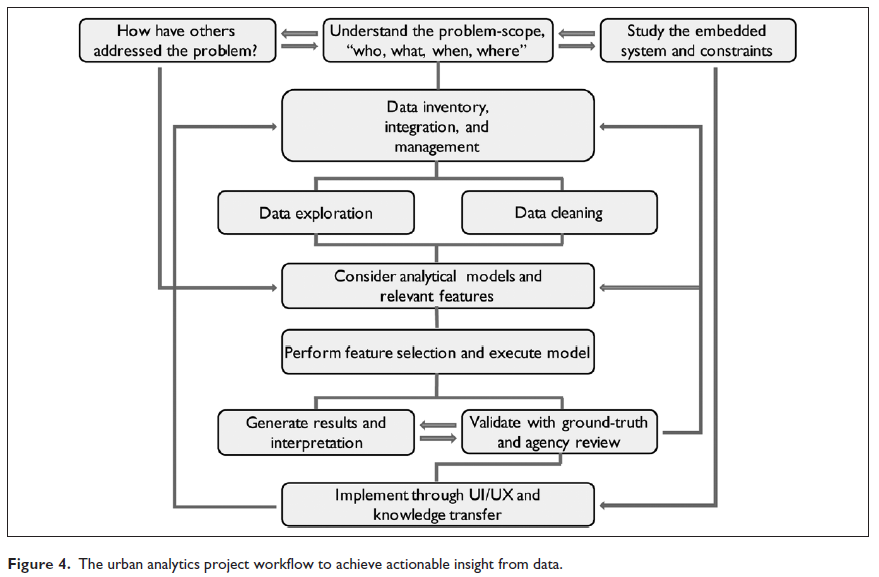
\includegraphics[width=0.4\textwidth]{Assets/data.PNG}
    \caption{Data and categorization of the model}
    \label{fig:datavars}
\end{figure}

\subsection{Networks}
\textbf{\citetitle{Chopra2014}}\par
\textcite{Chopra2014}, explore the dynamics of the Danish I.S. How did the symbiotic relationships evolved, what are the products or services exchanged. \par
Moreover, the aim of the study was also to deal with the resilience aspects of this I.S.
\textit{Since most of the industrial symbiotic networks are based on ad-hoc opportunities rather than strategic planning, gaining insight into disruptive scenarios is pivotal for understanding the balance of resilience and sustainability and developing heuristics for designing resilient IS networks. }
\textbf{CASE STUDY: } Kalundborg Industrial Symbiosis (KIS)

The present work focuses on understanding resilience as an emergent property of an IS network via a network-based approach. Scenarios are used to study resilience of the Case.

\textbf{\citetitle{Domenech2019}}\par
\textcite{Domenech2019}, \textit{The analysis is based on a combination of desk research, gathering of primary data from case studies, a survey to IS network facilitators (n=22) and in-depth interviews and focus groups (3) with IS practitioners, policy officers and industry representatives (n=25). The analysis identified pockets of IS activity across all Europe, although varying in nature, resources exchanged and scale and scope of the initiatives. The average size of the mapped networks is approx. 473 members, but the median is approx. 100 members, which indicates high variability of sizes. The geographical scope of the synergies also seems to be dependent upon the following factors: 1) the type of waste stream/by-product; 2) transport costs and 3) market value of secondary materials.}\par

\begin{figure}[h!]
    \centering
    \includegraphics[width=0.4\textwidth]{Assets/I.S. MAP.PNG}
    \caption{Map of case studies}
    \label{fig:casestudiesmap}
\end{figure}


\textit{The paper also discusses key obstacles facing IS development in Europe highlighting: 1) weakness of economic incentives given the low margin of IS projects associated to undeveloped secondary markets; 2) geographical variation of incentives and drivers, given differences in policy frameworks and support mechanisms (e.g. landfill tax levels) and 3) legislative issues that make transport over geographic boundaries extremely complex and administratively burdensome.}\par

The obstacles and determinants of I.S. are explored. The webpage of the project is down\par

From this paper a list of case studies and references can be extracted


\textbf{\citetitle{Ghali2019}}\par
\textcite{Ghali2019}, suggest that \textit{Industrial synergies join two or more organizations that initially functioned as independent economic actors that may originate from different sectors—together in order to share resources and exchange by-products for mutual environmental, financial, and social benefits for its participants. Industrial}.\par
\textit{In practice, the initiation of an industrial synergy, and particularly the identification of by-product compatibilities, relies on direct or facilitated knowledge and information sharing, which is essential for discovering industrial synergy opportunities.}\par
They propose a \textit{framework exploits the ability of the sematic web to enable the search for analogies between potential partners within a region or district and existing industrial synergies around the world.}\par
This requires (1) stakeholders to acknowledge their need to manage or acquire by-products, (2) data collection about waste and by-product flows and existing synergies, (3) potential synergy identification, and (4) some form of sharing data or contact between potential stakeholders.

\textbf{\citetitle{Morales2019}}\par
\textcite{Morales2019}, use the case study example of Altamira-Tampico in Mexico and study the I.S dynamics for a period of 20 years. \textit{The Industrial symbiosis emergence constitute a complex and dynamic process that we set in four different phases in this paper: Emergence, Regional efficiency, Regional learning, and Sustainable Industrial District.}\par
\textit{The industrial symbiosis at Altamira is depicted here as a centralized and ancillary industrial symbiosis embedding a socio-technical and environmental model, one of the most complete biophysical, social, and economic symbiotic case studies in Latin America.}\par



\begin{figure}[h!]
    \centering
    \includegraphics[width=0.4\textwidth]{Assets/Altamira.PNG}
    \caption{Map of Altamira-Tampico}
    \label{fig:altamiramap}
\end{figure}



\begin{figure}[h!]
    \centering
    \includegraphics[width=0.4\textwidth]{Assets/altamira dynamics.PNG}
    \caption{Typology of dynamics in Altamira}
    \label{fig:altamira_example}
\end{figure}




\textbf{\citetitle{Huang2019}}\par
\textcite{Huang2019}, produce a bibliometric analysis of the existing literature. Using social networks analysis of topics and author co-existing they produce a review of different aspects of I.S.\par
Their analysis reveals and helps to identify key words, journals and the importance of the topic. 

\textbf{\citetitle{Baldassarre2019}}\par
\textcite{Baldassarre2019}, see I.S as a way of bringing Competitive advantage to industry. In the paper it is discussed how Industrial Ecology and Circular Economy concepts contribute to Industrial Symbiosis.\par
The authors try to brig cohesion to the different definitions and explore the relationships between them.\par
In the paper the idea of how strategic design can contribute to help clusters of I.S.\par
They refer to a socio-technical process to develop I.S clusters.


\textbf{\citetitle{Herczeg2018}}\par
\textcite{Herczeg2018}, suggest that I.S has received little attention from the supply chain community.  \par

\begin{figure}[h!]
    \centering
    \includegraphics[width=0.8\textwidth]{Assets/case_studies.PNG}
    \caption{List of case studies}
    \label{fig:case_studies}
\end{figure}


They use the following framework.

\begin{figure}[h!]
    \centering
    \includegraphics[width=0.4\textwidth]{Assets/frame_gsupply.PNG}
    \caption{Frame work to explore Supply Chains}
    \label{fig:Supply chain explore}
\end{figure}


On the \textbf{organizational aspects of supply chain collaboration related to the supply chain integration} practices:\par
\textbf{Proposition (1a).} Collaborative strategic project definitions in IS networks require the development towards non-hazardous by-product synergies between environmentally sustainable processes.\par
\textbf{Proposition (1b).} Knowledge transfer and integration in IS net- works requires the establishment of a communication platform that connects local producers (or industries) with regulatory bodies, environmental experts, and community advocates.\par
Related to the \textbf{supply chain coordination practices,} we conclude the following:\par
\textbf{Proposition (2a).} Incentive alignment in IS networks requires the creation of a framework for sharing the costs, risks, and benefits of by- product synergies and emphasizing local economic, environmental, and social problems. \PAR 
\textbf{Proposition (2b).} Collective learning in IS networks requires the engagement of producers (industries) in learning about each others needs in order to guide them towards collaboration in solving strategic problems.\par
On the \textbf{operational aspects} of \textbf{supply chain collaboration}, related to the supply chain integration practice: \par
\textbf{Proposition (3a).} Production and delivery systems in IS networks require (i) the implementation of a local by-product collection and delivery system, and (ii) the integration of by-product treatment, storage, and reuse into regular operations.\par
\textbf{Proposition (3b). }Information systems for operational data in IS networks require the sharing of aggregated and temporal information on by-product flows with a network of current and potential partners.\par
\textbf{related to the supply chain coordination practices}:\par
\textbf{Proposition (4a).} Supply-demand agreements in IS networks require the development of agreements that facilitate redundancy in, and hence resilience of, the supply and demand of by-products in the IS network.\par
\textbf{Proposition (4b).} Logistical synchronization in IS networks requires the management of variability in quality and quantity of by-product flows as well as the matching of supply and demand.


\textbf{\citetitle{Song2018}}\par
\textcite{Song2018}, study the Gujiao I.S Eco park in China. Use network analysis to bring more efficiencies to the industrial park. The paper deals with some of the barriers that are faced to bring I.S. \par


\begin{figure}[h!]
    \centering
    \includegraphics[width=0.4\textwidth]{Assets/Gujiao.png}
    \caption{Gujiao}
    \label{fig:Gujiao}
\end{figure}


\textbf{\citetitle{Saavedra2018}}\par
\textcite{Saavedra2018}, try to uncover the importance of I.E to the concept of Circular Economy. According to their research, I.E bring 3 domains.: 1- Conceptual, 2-Technical, 3- Policy aspects.\par 

This is a bibliometric approach.

\textbf{\citetitle{Zhang2013}}\par
\textcite{Zhang2013}, explore the network properties of different I.S cases. They build on graph and network theory to analyse I.S relations. A total of 10 networks are studied. Yet, no geographical reference is introduced to the analysis. 


\begin{figure}[h!]
    \centering
    \includegraphics[width=0.4\textwidth]{Assets/IS Nets.PNG}
    \caption{IS networks}
    \label{fig:IS networks}
\end{figure}




\textbf{\citetitle{Zhu2013}}\par
\textcite{Zhu2013}, in this case the authors compare 2 cases of I.S, and determine the resilience of both cases. They use Netlogo to run a simulation of the relationships and explore what could happen to the industrial structure under different scenarios. Below there is an example  of one the analysis studied by the authors. \par



\begin{figure}[h!]
    \centering
    \includegraphics[width=0.4\textwidth]{Assets/disruptions.png}
    \caption{IS networks under disruptions}
    \label{fig:IS networks disrupted}
\end{figure}


The 2 cases studied are: \textit{The two cases selected are an industrial recycling network in Styria, Austria with 39 firms and 40 connections between the firms (Schwarz and Steininger, 1997), and a by-product and utility symbiosis network in Kwinana, Australia with 16 firms and 28 connections (Van Beers, 2008). We selected these cases because of their relative larger sizes than other reported cases. Network representations of the two cases are included as Supplemental material to this paper. The case of Styria includes more firms and is sparsely connected through a preferential attachment e or “rich-get-richer” e process, featuring the presence of more highly connected, anchor firms and their advantage in gaining connections. In contrast, the case of Kwinana has fewer firms but is more densely connected through a homogeneous attachment process, featuring the presence of fewer anchor firms and all firms equally likely to connect (Zhu and Ruth, submitted for publication). }



\textbf{\citetitle{Jung2013}}\par
\textcite{Jung2013}, evaluate the performance of Industrial Parks using Investment and Cash flows to determine their success. In this case I'm not very sure that this can be considered I.S. since no environmental factors are really taken into consideration. 



\textbf{\citetitle{Zhang2015a}}\par
\textcite{Zhang2015a}, take a closer look at the genesis and the definition of industrial symbiosis. \par


\begin{figure}[h!]
    \centering
    \includegraphics[width=0.4\textwidth]{Assets/examples.PNG}
    \caption{IS examples}
    \label{fig:IS examples}
\end{figure}


The paper concludes with some guidelines of future research. The lines proposed include:
1- Improve classification of the systems, \par 
2- Study changes in the system over time,  \par 
3 - Improve analyses of the relationships among members of the network.



\textbf{\citetitle{Lyons2007}}\par
\textcite{Lyons2007}, \textit{study the issue of geographic scale and loop closing for heterogeneous wastes through an analysis of the location and materials flows of a set of recycling, remanufacturing, recycling manufacturing, and waste treatment (RRWT) firms in Texas. The results suggest that there is no preferable scale at which loop closing should be organized. RRWT firms are ubiquitous and operate successfully throughout the settlement hierarchy. The cycling boundaries of RRWT firms are dependent primarily upon how and where their products are redirected to production processes rather than the firm’s location in the settlement hierarchy. In other words, loop closing is dominated by the spatial economic logic of the transactions of the firm involved. These results suggest that we cannot assign loop closing to any particular spatial scale a priori nor can we conceive of closing the loop via RRWT firms in terms of monolithic networks bounded in space or place with internal material flows} \par 

\textbf{Case study: TEXAS}



\textbf{\citetitle{Shi2010}}\par
\textcite{Shi2010}, produce a report of the Eco-Industrial Park in China. There is not a clear research question in the paper. Just showing numbers of the I.S experience. Also is important, because it helps to track down the historical evolution of the park.

\textbf{Case study: Tianjin in CHINA}



\textbf{\citetitle{Lombardi2005}}\par
\textcite{Lombardi2005}, discuss and stress the need of detailing the real benefits of Industrial Symbiosis. 


\textit{While industrial symbiosis is seen hypothetically as a win-win situation, there are few analyses of the economic and environmental consequences for the individual participants in multi-faceted exchanges. In this article, the nascent industrial symbiosis network in Guayama, Puerto Rico, is explored from environmental, economic, and regulatory perspectives of the individual participants and the community.}


\begin{figure}[h!]
    \centering
    \includegraphics[width=0.4\textwidth]{Assets/examples.PNG}
    \caption{IS examples}
    \label{fig:IS examples}
\end{figure}

\textbf{Case study: Guayama in PUERTO RICO}



\textbf{\citetitle{Liu2015}}\par
\textcite{Liu2015}, use a case study in China to propose a methodological framework to assess I.S relationships in the region. The paper seek to find potential opportunities
\textit{Implementing the three-level approach mainly shows that: (1) all the companies that implemented a cleaner production audit achieved economic and environmental benefits, (2) an existing symbiotic network was discovered, and (3) some potential symbiotic links were identified both at the inter-firm level and the regional level. Integrating cleaner production with industrial symbiosis, the relationship between the industrial symbiosis and its surrounding region, and the role of the government of implementing the three-level approach are discussed.}



\begin{figure}[h!]
    \centering
    \includegraphics[width=0.4\textwidth]{Assets/3level_approach.PNG}
    \caption{3 level approach to investigate I.S. relationships}
    \label{fig:3-stage approach}
\end{figure}

\textbf{Case study: Hai Hua Group (HHG) in CHINA}

\textbf{\citetitle{Trokanas2014}}\par
\textcite{Trokanas2014}, propose a semantic i/o matching for waste. Using an ontological approach wastes from one industry are matched to another. 

\textbf{This paper is quite complex. Uses semantics, ontology to match between inputs and outputs. Maybe would be worthy to explore how they did this more in detail later on. Specially when they make reference to geographical data.}




\textbf{\citetitle{Posch2011}}\par
\textcite{Posch2011}, writes the editorial of the special issue and introduces a set of articles of Industrial Symbiosis. Here the idea that I.S is much more than actual exchanges is stressed. The article introduces more concepts to the industrial symbiosis domain. \par
For instance, the idea of \textit{'Bounded Rationality'}, is borrowed from politics and economics to highlight the fact that the choices are restricted to a set of options, and that there is a need to expand them. \par
The article or selection of them, focuses on the decision making process and suggest that in order to talk about I.S. reducing the environmental pressure is a must.



\textbf{\citetitle{Cerceau2014}}\par
\textcite{Cerceau2014},






\textbf{\citetitle{Domenech2011b}}\par
\textcite{Domenech2011b},






\textbf{\citetitle{Boix2015}}\par
\textcite{},



\textbf{\citetitle{Aviso2015}}\par
\textcite{},


\textbf{\citetitle{Chopra}}\par
\textcite{},


\textbf{\citetitle{Mirata2004}}\par
\textcite{},


\textbf{\citetitle{Guo2016}}\par
\textcite{}